\documentclass[uplatex]{jsarticle}
\usepackage[dvipdfmx]{graphicx}
\usepackage{ascmac}
\usepackage{listings}
\usepackage{amsmath}
\usepackage{bm}
\usepackage{cases}

\DeclareMathOperator*{\minimize}{minimize}


\title{人工知能 課題番号1「人工知能の実現可能性について考察せよ」}
\author{工学部電子情報工学科 03-175001 浅井明里}

\makeatletter
\def\maketitle{%
  \null
  \thispagestyle{empty}%
  \vfill
  \begin{center}\leavevmode
    \normalfont
    {\LARGE \@title\par}%
    \vskip 1cm
    {\Large \@author\par}%
    \vskip 1cm
    {\Large \@date\par}%
  \end{center}%
  \vfill
  \null
  \@thanks%\vfil\null
  \cleardoublepage
  }
\makeatother


\title{人工知能 課題番号5「制約従属問題をTMSを用いて解く」}
\author{工学部電子情報工学科 03-175001 浅井明里}
\date{\today}

\begin{document}
\maketitle

\section{TMSとは}
数学的な論理では仮定は常に正しいとされるが、現実世界においては状況が変化する等により、
新しい事実が刻一刻と生まれ、これまでの結論を修正しなくてはいけないことが多々ある。たとえば、
「明日はおそらく台風が接近するため天候が大きく荒れるはずだ」「天候が大きく荒れている時に通学をするのは危険なため、
おそらく明日の午前の授業は休講となるだろう」「つまり明日の午前は休講となるため、大学に行く必要がない」と推定したとしても、
実際に次の日に台風が接近しなかった場合、授業は休講にならず、我々は大学に行かなくてはいけなくなる。
こういった非単調論理推論の代表例にTMS(Truth-mentenace system)というシステムがある。

TMSにおいて、データの状態には以下の二種類が存在する。
\begin{itemize}
  \item In状態 : 現在のデータに対応する命題を信じている
  \item Out状態 : 現在のデータに対応する命題を信じている
\end{itemize}
TMSで重要となるのは「矛盾」の解消であり、
矛盾が発生した際には、矛盾を起こす原因のデータをOutとし、代わりに他のデータをInすることで、
仮説のIn/Out状態を修正して真理を維持する。

\section{TMSで領域4色塗り分け問題を解く}
本レポートでは、いくつかの領域に分割された地図を4色で塗り分ける制約従属問題をTMSで解いていく。
今回は図1で示された地図を4色で塗り分ける場合を考える。
\begin{figure}
  \begin{center}
    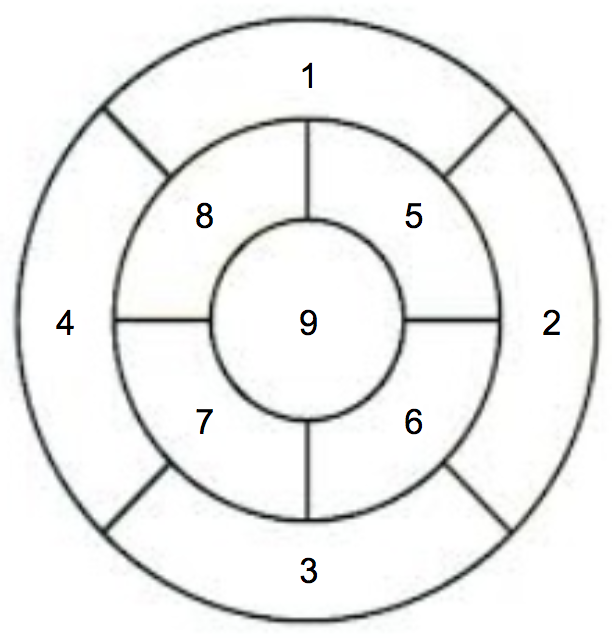
\includegraphics[width=8cm]{img/color_default.png}
    \caption{4色塗り分け問題の初期状態}
  \end{center}
\end{figure}

\subsection{仮説知識、NoGood知識を制約条件から求める}
まず、TMSのデータベースを構成する。ある地図を「赤」「青」「黄」「緑」の四色で塗り分ける時、以下のような制約が存在する。
\begin{itemize}
  \item それぞれの領域は必ずどれか一色で塗られており、終末状態において白色のまま、もしくは二色で一つの領域が塗られてはならない。
  \item 隣り合う領域は異なる色で塗られていなくてはいけない。
\end{itemize}
この制約条件に基づき、TMSの仮説知識のデータを構築する。
$n$分割された領域について、それぞれ「領域$k(1 \leq n)$」と名付け、
「赤」「青」「黄」「緑」について、「R」「B」「Y」「G」とし、例えば「領域1が赤色で塗られている」
という知識を「R1」と表すこととする。また、どの色にも塗り分けられていない状態を「白色」すなわち「W」として
仮に領域1がどの色にも塗り分けられていない時、この状態を「W1」とする。

この表記を用いて、まず「ある領域はどれか一色で塗られている、そうでなければ白色のままである」という仮説知識を、領域1について構成する。
\begin{itemize}
  \item R1 : SL : {IN:{}, Out:{G1, B1, Y1}}
  \item G1 : SL : {IN:{}, Out:{R1, B1, Y1}}
  \item B1 : SL : {IN:{}, Out:{R1, G1, Y1}}
  \item Y1 : SL : {IN:{}, Out:{R1, G1, B1}}
  \item W1 : SL : {IN:{}, Out:{R1, G1, B1, Y1}}
\end{itemize}
他の8つの領域についても同様の仮説知識が成立するため、計$5\times9 = 45$個の仮説知識が構成できる。

次に、No-Good知識について考えてみる。この4色塗り分け問題におけるNo-Goodな状態とは、
「彩色されていない領域が地図上にある」もしくは「隣り合う領域が同じ色で彩色されている」という状態である。
ある領域が彩色されていないというNo-Good状態は以下の9通り存在する。
\begin{itemize}
  \item NG-W1:{NoGood:{W1}}
  \item NG-W2:{NoGood:{W2}}
  \item NG-W3:{NoGood:{W3}}
  \item NG-W4:{NoGood:{W4}}
  \item NG-W5:{NoGood:{W5}}
  \item NG-W6:{NoGood:{W6}}
  \item NG-W7:{NoGood:{W7}}
  \item NG-W8:{NoGood:{W8}}
  \item NG-W9:{N0Good:{W9}}
\end{itemize}

また、領域1から9について、隣り合っている領域は表1の通りである。
\begin{table}[htb]
  \begin{center}
    \caption{それぞれの領域に隣接する領域と、No-Goodの例}
  \begin{tabular}{|l|c|c|} \hline
    領域 & 隣接する領域 & No-Goodの例\\ \hline\hline
    1 & 2, 4, 5, 8 & NG-R12 : {NoGood:{R1, R2}} \\
    2 & 1, 3, 5, 6 & NG-R23 : {NoGood:{R2, R3}} \\
    3 & 2, 4, 6, 7 & NG-R34 : {NoGood:{R3, R4}}\\
    4 & 1, 3, 7, 8 & NG-R47 : {NoGood:{R4, R7}} \\
    5 & 1, 2, 6, 8, 9 & NG-R56 : {NoGood:{R5, R6}} \\
    6 & 2, 3, 5, 7, 8 & NG-R67 : {NoGood:{R6, R7}} \\
    7 & 3, 4, 6, 8, 9 & NG-R78 : {NoGood:{R7, R8}} \\
    8 & 1, 4, 5, 7, 9 & NG-R89 : {NoGood:{R8, R9}} \\
    9 & 5, 6, 7, 8 & NG-R95 : {NoGood:{R9, R5}} \\ \hline
  \end{tabular}
\end{center}
\end{table}
No-Goodの例は隣接する領域の組み合わせの数が20通り存在し、それぞれについて4色考える必要があるので $20 \times 4= 80$種類存在し、
いずれかの領域が白色となるNo-Goodと合わせて計89種類のNo-Good状態が存在することになる。

\subsection{4色塗り分け問題に対するTMS解法の流れ}
TMSにより隣接する領域の4色塗り分け問題を解くには以下のようなステップが必要である。
\begin{enumerate}
 \item 全ての仮説知識、NoGood知識(制約条件)を設定する。
 \item いずれの仮説知識もOutの初期状態から開始する。
 \item ここからランダムに仮説知識の要素をOutから選択しInとする。
 \item NoGood知識と照らし合わせて矛盾が生じるか確認する。矛盾がなければ次の領域を塗り分けていく。
 \item 矛盾がIn状態となった場合には、この解消のためサポートリストのIn状態に含まれる要素がランダムに選ばれ、
 そのサポートリストのOutに含まれる要素をランダムに選び、矛盾を生んだ仮説知識についてはOutとする。
 \item これを全ての領域が塗り終わるまで繰り返す。
 \end{enumerate}
今回は、このステップを実行し4色塗り分け問題を解く、TMSColorSolver.cppというプログラムを作成しその結果を観測した。

\subsection{4色塗り分けプログラムの実行結果}
前述のプログラムを以下のコマンドにより実行した。
\begin{lstlisting}[basicstyle=\ttfamily\footnotesize, frame=single]
$ g++ -std=c++11 TMSSolver.cpp
$ ./a.out
\end{lstlisting}
出力結果については本レポートの最後のページに添付した。

\begin{enumerate}
  \item まず、初期状態からW1がInに追加される。
  \item W1はNoGood状態として定義されているため、Solverはこの矛盾を解消するため、OutからR1を取り出す。
  \item W1がOutへ、R1はInに追加される。
  \item 同様にW2、W3も一旦Inに追加された後、NoGood解消のため別の仮説知識がOutから取り出される。
  \item 領域2、3共に黄色で塗られ、これは$\rm{Y}_{2,3}$というNoGood状態であるため、
  OutからG2がInに入り、領域2は緑色に塗り替えられる。
  \item 領域4についても同様の手順で色付けがされ、結果として領域1から4までが一旦図3のように塗り分けられる。
  \item 領域5が一旦赤で塗られるが、$\rm{R}_{2,5}$となりNoGood状態であるため、OutからB5が取り出され、領域5が青く塗り変えられる。
  \item OutからB6が取り出されるが、これは$\rm{B}_{5,6}$となるため、OutからG5が取り出されInとなる。
  \item 領域1と5共に緑で塗られることとなり、NoGood状態となるため、outからR5が取り出される。
  \item 同様の手順で矛盾を解消していき、結果的に領域6までが図3のように塗り分けられた。
  \item 領域7も同様の手順で塗り分けていく。まずR7がOutから取り出されるが、これは$\rm{R}_{4,7}$というNoGood状態となるため、
  B4が取り出され、領域4が青に塗り替えられるがこれは$\rm{B}_{4,1}$という別のNoGood状態となる。
  \item このNoGoodの解消のため、G1, R2, G2, B1, G4が順にOutからInに取り出され、結果として領域7までが図4のように塗り分けられる。
  \item 残り2領域についても、ランダムにOutから仮説知識を取り出し、仮にNoGoodがInに入った際には矛盾の解消のため異なる仮説知識をOutから取り出す作業を続け、
  最終的に塗り分け結果は図5のようになった。
\end{enumerate}
今回は9領域の4色塗り分けについて、TMSから正しく正解を導くことができた。TMSはデータの相互依存関係を保持することにより、
矛盾が怒った時にその矛盾に関連するデータのIn/Out状態だけを変更して矛盾を解消することができるという特長をうまく体現していると言える。
一方で、矛盾が生じた際にどのデータをIn/Outにするかはランダムに決定されるために、やや非効率とも思える選択をしている場面も見受けられた。
例えば、最終領域を塗り分ける際、人間であれば隣接する4領域で使用されていない緑で塗れば完成するとすぐに判断することができるであろうが、

また、今回のプログラムでは一度ランダムにB9がInとなったために、結果として生じた多くの矛盾の解消のため非効率な計算が行われることとなった。
今回のような少ない領域の塗り分け問題についてはTMSでも十分正しい解答を導くことができるが、
TMSのようにランダムに矛盾のない解を見つけようとするアルゴリズムは問題がより複雑により多くの状態が想定できる場合にはどれくらいの計算が必要なのか
予測できないという問題がある。

\begin{figure}[htbp]
\begin{minipage}{0.5\hsize}
 \begin{center}
  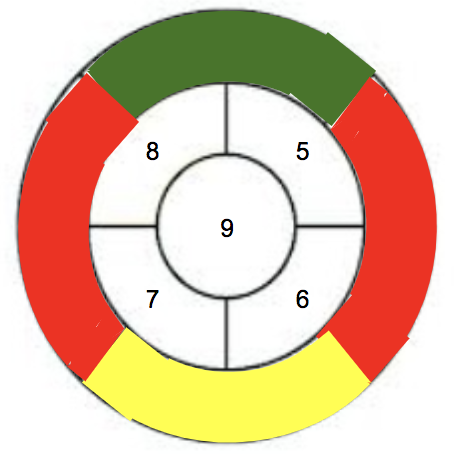
\includegraphics[width=70mm]{img/step1.png}
 \end{center}
 \caption{6ステップ目終了時の塗り分けの様子}
 \label{fig:one}
\end{minipage}
\begin{minipage}{0.5\hsize}
 \begin{center}
  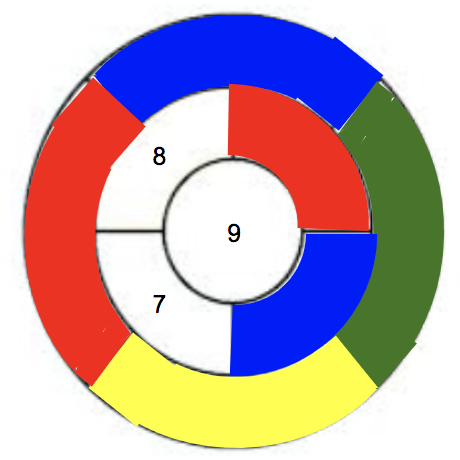
\includegraphics[width=70mm]{img/step2.png}
 \end{center}
 \caption{10ステップ目終了時の塗り分けの様子}
 \label{fig:two}
\end{minipage}
\end{figure}
\begin{figure}[htbp]
\begin{minipage}{0.5\hsize}
 \begin{center}
  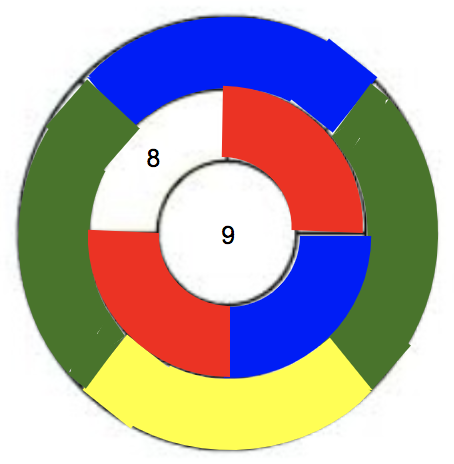
\includegraphics[width=70mm]{img/step3.png}
 \end{center}
 \caption{12ステップ目終了時の塗り分けの様子}
 \label{fig:one}
\end{minipage}
\begin{minipage}{0.5\hsize}
 \begin{center}
  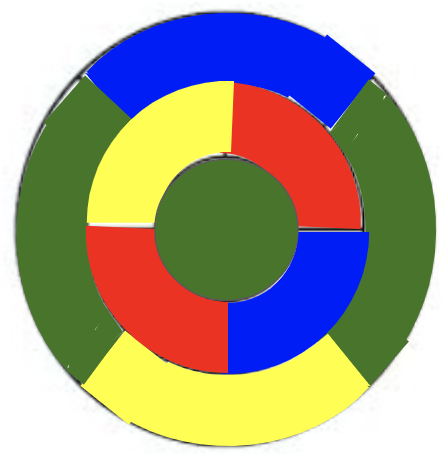
\includegraphics[width=70mm]{img/step4.png}
 \end{center}
 \caption{最終的な塗り分けの結果}
 \label{fig:two}
\end{minipage}
\end{figure}


\begin{thebibliography}{9}
  \bibitem{imageNet} 伊庭斉志,
    『人工知能と人工生命の基礎』, オーム社 , 2013.
% http://www.orsj.or.jp/~archive/pdf/bul/Vol.32_09_606.pdf
\end{thebibliography}

\clearpage
以下はTMSColorSolver.cppの出力結果である。

\begin{lstlisting}[basicstyle=\ttfamily\footnotesize, frame=single]
step : W1 turned to In
NG_W1 need to be resolved
step : W1 turned out, R1 turned in
step : W2 turned to In
NG_W2 need to be resolved
step : W2 turned out, Y2 turned in
step : W3 turned to In
NG_W3 need to be resolved
step : W3 turned out, Y3 turned in
NG_Y23 need to be resolved
step : Y2 turned out, G2 turned in
step : W4 turned to In
NG_W4 need to be resolved
step : W4 turned out, R4 turned in
NG_R41 need to be resolved
step : R1 turned out, G1 turned in
NG_G12 need to be resolved
step : G2 turned out, R2 turned in
step : W5 turned to In
NG_W5 need to be resolved
step : W5 turned out, R5 turned in
NG_R25 need to be resolved
step : R5 turned out, B5 turned in
step : W6 turned to In
NG_W6 need to be resolved
step : W6 turned out, B6 turned in
NG_B56 need to be resolved
step : B5 turned out, G5 turned in
NG_G15 need to be resolved
step : G5 turned out, R5 turned in
NG_R25 need to be resolved
step : R2 turned out, Y2 turned in
NG_Y23 need to be resolved
step : Y2 turned out, G2 turned in
NG_G12 need to be resolved
step : G1 turned out, R1 turned in
NG_R41 need to be resolved
step : R1 turned out, B1 turned in
step : W7 turned to In
NG_W7 need to be resolved
step : W7 turned out, R7 turned in
NG_R47 need to be resolved
step : R4 turned out, B4 turned in
NG_B41 need to be resolved
step : B1 turned out, G1 turned in
NG_G12 need to be resolved
step : G2 turned out, R2 turned in
NG_R25 need to be resolved
step : R2 turned out, G2 turned in
NG_G12 need to be resolved
step : G1 turned out, B1 turned in
NG_B41 need to be resolved
step : B4 turned out, G4 turned in
step : W8 turned to In
NG_W8 need to be resolved
step : W8 turned out, Y8 turned in
step : W9 turned to In
NG_W9 need to be resolved
step : W9 turned out, B9 turned in
NG_B69 need to be resolved
step : B6 turned out, Y6 turned in
NG_Y36 need to be resolved
step : Y6 turned out, G6 turned in
NG_G26 need to be resolved
step : G6 turned out, B6 turned in
NG_B69 need to be resolved
step : B6 turned out, Y6 turned in
NG_Y36 need to be resolved
step : Y6 turned out, B6 turned in
NG_B69 need to be resolved
step : B9 turned out, G9 turned in
step : Successfully finished coloring!
\end{lstlisting}

\end{document}
